\section{Introduction to Network Diversion}

Now that we have an algorithm for \textsc{Shortest Odd Path}, we will use it to solve a much more useful problem:

\problem
{Network Diversion}
{a weighted graph $G := (V, E, \from, \too, \weight)$, two vertices $s,t \in V$, and a \emph{diversion edge}~$d~\in~E$}
{a \emph{diversion set} $D \subseteq E$ of minimum weight such that all $s$-$t$-paths in~$(V,~E~\setminus~D,~\from,~\too,~\weight)$ must go through $d$}

A diversion set may also equivalently be defined as a minimal $s$-$t$-cut that includes~$d$. If all edges from the diversion set are deleted except~$d$, then~$d$ is the bridge between what would otherwise be two separate components and all $s$-$t$-paths must go through $d$. \textsc{Network Diversion} can then be restated as the quest to find a \emph{minimum} minimal $s$-$t$-cut that includes $d$. Both definitions are equivalent and yield the same optimum results, and being able to switch between formulations of the problem makes it easier to solve them.

See \Cref{figure:diversion-attempts} for examples. \Cref{subfigure:invalid-diversion1} and \Cref{subfigure:invalid-diversion2} show incorrect attempts at diversions, while \Cref{subfigure:valid-diversion} shows a valid diversion.

\begin{figure}[H]
    \centering
    \begin{subfigure}{.3\textwidth}
        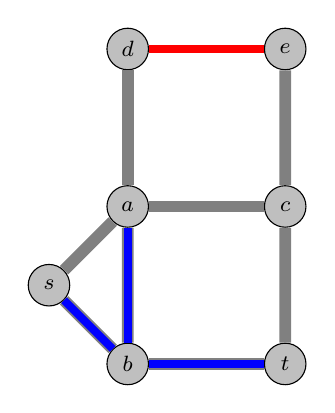
\begin{tikzpicture}
            \tikzstyle{every node}=[circle, fill=lightgray, draw=black, inner sep=2pt, minimum size=1.5em, font=\footnotesize, text=black]
            \tikzstyle{edge}=[gray, line width=1.5mm]
       
            \node (s) at (0,1) {$s$};
            \node (a) at (1,2) {$a$};
            \node (b) at (1,0) {$b$};
            \node (t) at (3,0) {$t$};
            \node (d) at (1,4) {$d$};
            \node (c) at (3,2) {$c$};
            \node (e) at (3,4) {$e$};

            \draw[edge] (b) -- (s) -- (a) -- (b) -- (t) -- (c) -- (e);
            \draw[edge] (c) -- (a) -- (d);
       
            \tikzstyle{edge}=[red, line width=1mm]
            \draw[edge] (d) -- (e);

            \tikzstyle{edge}=[blue, line width=1mm]
            \draw[edge] (s) -- (b);
            \draw[edge] (a) -- (b) -- (t);
        \end{tikzpicture}
        \caption{Invalid, there are still paths that don't go through the diversion edge}
        \label{subfigure:invalid-diversion1}
    \end{subfigure}\hfill%
    \begin{subfigure}{.3\textwidth}
        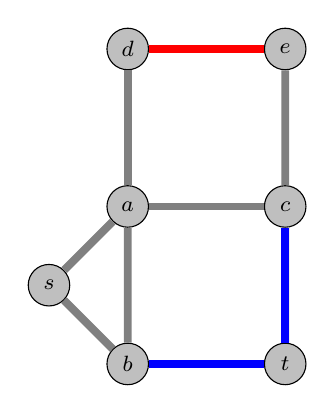
\begin{tikzpicture}
            \tikzstyle{every node}=[circle, fill=lightgray, draw=black, inner sep=2pt, minimum size=1.5em, font=\footnotesize, text=black]
            \tikzstyle{edge}=[gray, line width=1mm]
       
            \node (s) at (0,1) {$s$};
            \node (a) at (1,2) {$a$};
            \node (b) at (1,0) {$b$};
            \node (t) at (3,0) {$t$};
            \node (d) at (1,4) {$d$};
            \node (c) at (3,2) {$c$};
            \node (e) at (3,4) {$e$};

            \draw[edge] (b) -- (s) -- (a) -- (b) -- (t) -- (c) -- (e);
            \draw[edge] (c) -- (a) -- (d);
       
            \tikzstyle{edge}=[red, line width=1mm]
            \draw[edge] (d) -- (e);

            \tikzstyle{edge}=[blue, line width=1mm]
            \draw[edge] (b) -- (t);
            \draw[edge] (c) -- (t);
        \end{tikzpicture}
        \caption{Invalid, the diversion set also blocks all paths that use the diversion edge}
        \label{subfigure:invalid-diversion2}
    \end{subfigure}\hfill%
    \begin{subfigure}{.3\textwidth}
        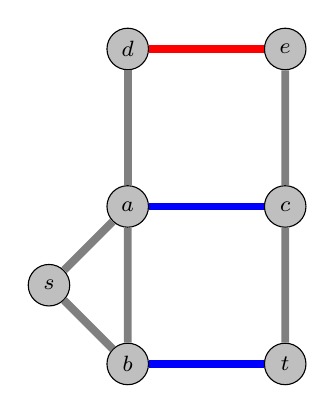
\begin{tikzpicture}
            \tikzstyle{every node}=[circle, fill=lightgray, draw=black, inner sep=2pt, minimum size=1.5em, font=\footnotesize, text=black]
            \tikzstyle{edge}=[gray, line width=1mm]
       
            \node (s) at (0,1) {$s$};
            \node (a) at (1,2) {$a$};
            \node (b) at (1,0) {$b$};
            \node (t) at (3,0) {$t$};
            \node (d) at (1,4) {$d$};
            \node (c) at (3,2) {$c$};
            \node (e) at (3,4) {$e$};

            \draw[edge] (b) -- (s) -- (a) -- (b) -- (t) -- (c) -- (e);
            \draw[edge] (c) -- (a) -- (d);
       
            \tikzstyle{edge}=[red, line width=1mm]
            \draw[edge] (d) -- (e);

            \tikzstyle{edge}=[blue, line width=1mm]
            \draw[edge] (b) -- (t);
            \draw[edge] (a) -- (c);
        \end{tikzpicture}
        \caption{Valid, the diversion set funnels all traffic through the diversion}
        \label{subfigure:valid-diversion}
    \end{subfigure}
    \caption{Valid and invalid diversions, attempting to force all $s$-$t$ paths to go through the diversion edge in red by deleting the diversion set in blue.}
    \label{figure:diversion-attempts}
\end{figure}

Unlike with \textsc{Shortest Odd Path}, it is much easier to come up with practical applications of \textsc{Network Diversion}. Consider a communications network of machines that communicate offline, where you, a spy, can intercept all messages between two specific machines. How can you through outages and other diversions force all traffic in the network to go through where you can intercept the messages? Or for a more direct example: consider a network of roads and bridges, the knowledge that the enemy wants to move troops and supplies from one point to another, and a specific bridge where you are especially prepared to ambush them. How can you with the least amount of artillery destroy bridges to force the enemy to move through your ambush?

Initially, finding a minimum minimal $s$-$t$-cut that includes a specific edge may seem like yet another variation of the well-known minimum $s$-$t$-cut problem, of which we have numerous excellent polynomial-time algorithms. Yet, this is considerably harder to solve correctly. If we just use a normal flow algorithm like Edmonds-Karp \cite{source:edmonds-karp-algorithn}, we are very likely to end up with a minimum cut that does \emph{not} include the diversion edge, like in \Cref{subfigure:invalid-diversion2}. And if we force the flow algorithm to use the diversion edge, we are likely to end up with a cut that is not minimal, a cut where we might as well drop the diversion edge from the set and still have a cut, like in \Cref{subfigure:invalid-diversion2}.

In fact, \cite{source:theoretical-and-computational-advances-for-network-diversion} have shown that \textsc{Network Diversion} is NP-complete on directed graphs, even without cycles or weights. Whether \textsc{Network Diversion} can be solved in polynomial time on undirected graphs is still an open problem. \cite{source:theoretical-and-computational-advances-for-network-diversion} have found polynomial-time algorithms for the special case where the input graph is $s$-$t$-planar, meaning that the graph can be embedded such that $s$ and $t$ are adjacent to the outside face, but whether there is a polynomial-time algorithm for planar graphs in the general case is still an open problem.

Until now. We will present the first-ever polynomial-time algorithm that solves \textsc{Network Diversion} in undirected planar graphs. It will also work with weighted edges, as long as the weights are non-negative. Many graphs based on physical structures are planar. In the example of roads and bridges, having two roads cross without a crossroad is usually inefficient and more costly, so such networks are very often planar. The costs associated with cutting an edge or blowing up a bridge are usually non-negative, too. So even if we do not solve \textsc{Network Diversion} in the most general case, solving it for planar graphs of non-negative edges is not far from it in practice.
